\documentclass[calcdimensions,landscape,letterpaper]{powersem}
\usepackage{color}
\usepackage[pdftex]{thumbpdf} % For thumbnails
\usepackage[pdftex]{hyperref} % For links.
\usepackage[display,coloremph,whitebackground]{texpower} % colormath
\usepackage{fixseminar}
\usepackage{tpslifonts}
\usepackage[pdftex,final]{graphicx} % For including graphics.
\usepackage[utf8]{inputenc}
\usepackage{minted}
\usepackage{amsmath}
\usepackage{amssymb}
\usepackage{eurosym}
\usepackage{booktabs} % rules in tables
\usepackage{multirow} % multi-row cells
\usepackage{rotating} % text rotation

\title{The SOLID Principles}
\author{Jan Wedekind}
\date{Tuesday, Jan 21st 2025}

\DeclareGraphicsExtensions{.jpg,.pdf,.png}
\pdfcompresslevel=9

\hypersetup{
   pdftitle          = {\thetitle},
   pdfsubject        = {Short presentation about the SOLID software design principles},
   pdfauthor         = {Jan Wedekind},
   pdfkeywords       = {solid, software, design},
   pdfcreator        = {okular},
   pdfproducer       = {LaTeX with hyperref and thumbpdf},
   bookmarksopen     = false,
   bookmarksnumbered = true,
   colorlinks        = true,
}

\DeclarePanel{top}{
  \begin{picture}(0,0)
    \put(-3, -293){\resizebox*{\pdfpagewidth}{\pdfpageheight}{
\includegraphics{slide.png}}}
    \put(-10,-20){\parbox[c]{.9\textwidth}{\center\large\bf\thecurrentheading}}
  \end{picture}
}

\DeclarePanel{bottom}{
  \begin{picture}(0,0)
    \put(0,15){\parbox[c]{.98\pdfpagewidth}{\tiny\thedate\hfill\theslide/22}}
  \end{picture}
}

\slidesmag{4}
\backgroundstyle{none}
\slideframe{none}
\pagestyle{empty}

\mklength{\slideleftmargin}{-2cm}
\mklength{\sliderightmargin}{-2cm}
\mklength{\slidetopmargin}{2.0cm}
\mklength{\slidebottommargin}{1.5cm}

\renewcommand{\currentpagevalue}{\value{slide}}
\newcommand{\thecurrentheading}{}
\newcommand{\heading}[1]{\renewcommand{\thecurrentheading}{#1}}
\newcommand{\subheading}[1]{\concept{#1}}

\begin{document}

\begin{slide}
  \pdfbookmark[1]{\thetitle}{title}
  \heading{\ }
  \begin{center}
    \maketitle
  \end{center}
\end{slide}

\begin{slide}
  \pdfbookmark[1]{Motivation}{motivation}
  \heading{Motivation}
  \begin{center}
    \begin{minipage}[c]{.5\textwidth}
      \begin{center}
        \resizebox*{.93\textwidth}{!}{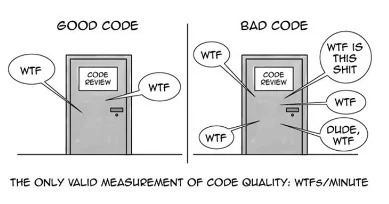
\includegraphics{wtf-per-minute}}\bigskip\\
        Find guiding design principles to maintain software quality over time.
      \end{center}
    \end{minipage}
  \end{center}
\end{slide}

\begin{slide}
  \pdfbookmark[1]{Software Rot}{software-rot}
  \heading{Software Rot}
  \begin{center}
    \textbf{Symptoms of rotting software design:}\footnote{Robert C. Martin: \href{https://staff.cs.utu.fi/~jounsmed/doos_06/material/DesignPrinciplesAndPatterns.pdf}{Design Principles and Design Patterns}}
    \begin{itemize}
      \item \textbf{Rigidity}: software difficult (a lot of work) to change
      \item \textbf{Fragility}: changes easily break the software
      \item \textbf{Immobility}: it is easier to rewrite than reuse parts
      \item \textbf{Viscosity}: design preserving methods are harder to employ than hacks
    \end{itemize}
  \end{center}
\end{slide}

\begin{slide}
  \pdfbookmark[1]{Aims}{aims}
  \heading{Aims}
  \begin{center}
    \textbf{In contrast we want to achieve the following:}\footnote{Robert C. Martin: \href{https://staff.cs.utu.fi/~jounsmed/doos_06/material/DesignPrinciplesAndPatterns.pdf}{Design Principles and Design Patterns}}\medskip\\
    \begin{minipage}[c]{.65\textwidth}
      \begin{itemize}
        \item Keep software application \textbf{flexible}
        \item Keep software application \textbf{robust}
        \item Keep software application \textbf{reusable}
        \item Keep software application \textbf{developable}
      \end{itemize}
    \end{minipage}
  \end{center}
\end{slide}

\begin{slide}
  \pdfbookmark[1]{SOLID Authors}{solid-authors}
  \heading{SOLID Authors}
  \begin{center}
    \begin{minipage}[b]{.25\textwidth}
      \begin{center}
        \resizebox*{.93\textwidth}{!}{
\includegraphics{robert-martin}}\\
        Robert C. Martin\bigskip\\
      \end{center}
    \end{minipage}
    \begin{minipage}[b]{.7\textwidth}
      \begin{itemize}
        \item Author of \href{https://www.informit.com/store/clean-code-a-handbook-of-agile-software-craftsmanship-9780132350884}{Clean Code}, \href{https://www.informit.com/store/functional-design-principles-patterns-and-practices-9780138176396}{Functional Design}, and more books
        \item Author of \href{https://staff.cs.utu.fi/~jounsmed/doos_06/material/DesignPrinciplesAndPatterns.pdf}{Design Principles and Design Patterns} paper based on his experience and on work by Bertrand Meyer, Barbara Liskov, and Erich Gamma et al.
        \item \url{http://cleancoder.com/}
      \end{itemize}
    \end{minipage}\\\rule{.95\textwidth}{1pt}
    \begin{minipage}[b]{.25\textwidth}
      \begin{center}
        \resizebox*{.93\textwidth}{!}{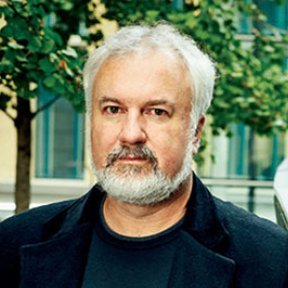
\includegraphics{michael-feathers}}\\
        Michael Feathers
      \end{center}
    \end{minipage}
    \begin{minipage}[b]{.7\textwidth}
      \begin{itemize}
        \item Author of \href{https://www.informit.com/store/working-effectively-with-legacy-code-9780131177055}{Working Effectively With Legacy Code}
        \item Summarized Robert C. Martin's paper using the SOLID acronym
        \item \url{https://www.r7krecon.com/}
      \end{itemize}
    \end{minipage}
  \end{center}
\end{slide}

\begin{slide}
  \pdfbookmark[1]{The SOLID Principles}{solid-principles}
  \heading{The SOLID Principles}
  \begin{center}
    \begin{Large}
      \begin{minipage}[c]{.6\textwidth}
        \begin{enumerate}
          \item \textbf{S}ingle responsibility
          \item \textbf{O}pen-closed
          \item \textbf{L}iskov substitution
          \item \textbf{I}nterface segregation
          \item \textbf{D}ependency inversion
        \end{enumerate}
      \end{minipage}
    \end{Large}
  \end{center}
\end{slide}

\begin{slide}
  \pdfbookmark[1]{Single Responsibility}{single-responsibility}
  \pdfbookmark[2]{Before}{single-responsibility-before}
  \heading{Single Responsibility - Before}
  \begin{center}
    \begin{minted}{clojure}
(defn adults-to-html [people]
  (str
    "<ul>\n"
    (apply str
           (for [person people :when (>= (:age person) 18)]
                (str "<li>" (:name person) "</li>\n")))
    "</ul>"))
; ...
(def page (adults-to-html people))
    \end{minted}
  \end{center}
\end{slide}

\begin{slide}
  \pdfbookmark[2]{After}{single-responsibility-after}
  \heading{Single Responsibility - After}
  \begin{center}
    \begin{minted}{clojure}
(defn select-adults [people]
  (filter
    (fn [person] (>= (:age person) 18))
    people))

(defn people-to-html [people]
  (str
    "<ul>\n"
    (apply str
           (for [person people]
             (str "<li>" (:name person) "</li>\n")))
    "</ul>"))
; ...
(def page (people-to-html (select-adults people)))
    \end{minted}
  \end{center}
\end{slide}

\begin{slide}
  \pdfbookmark[1]{Open-Closed}{open-closed}
  \pdfbookmark[2]{Before}{open-closed-before}
  \heading{Open-Closed - Before}
  \begin{center}
    \begin{minted}{clojure}
(defn total-area [shapes]
  (reduce +
    (map
      (fn [shape]
        (case (:type shape)
          ::circle (* Math/PI (:radius shape) (:radius shape))
          ::rectangle (* (:width shape) (:height shape))))
      shapes)))
    \end{minted}
  \end{center}
\end{slide}

\begin{slide}
  \pdfbookmark[2]{After}{open-closed-after}
  \heading{Open-Closed - After}
  \begin{center}
    \begin{minted}{clojure}
(defmulti area :type)

(defmethod area ::circle [shape]
  (* Math/PI (:radius shape) (:radius shape)))

(defmethod area ::rectangle [shape]
  (* (:width shape) (:height shape)))

(defn total-area [shapes]
  (reduce +
    (map area shapes)))
    \end{minted}
  \end{center}
\end{slide}

\begin{slide}
  \pdfbookmark[1]{Liskov-Substitution}{liskov-substitution}
  \pdfbookmark[2]{Before}{liskov-substitution-before}
  \heading{Liskov-Substitution - Before}
  \begin{center}
    \begin{minted}{clojure}
(defmulti set-width (fn [x width] (:type x)))
(defmethod set-width ::rectangle [x width]
  (assoc x :width width))
(defmethod set-width ::square [x width]
  (assoc x :width width :height width))

(defmulti set-height (fn [x height] (:type x)))
(defmethod set-height ::rectangle [x height]
  (assoc x :height height))
(defmethod set-height ::square [x height]
  (assoc x :width height :height height))

(defmulti area :type)
(defmethod area ::rectangle [x] (* (:width x) (:height x)))
(derive ::square ::rectangle)
    \end{minted}
  \end{center}
\end{slide}

\begin{slide}
  \pdfbookmark[2]{Contracts}{liskov-substitution-contracts}
  \heading{Liskov-Substitution - Contracts}
  \begin{center}
    ``The Liskov Substitution Principle states, among other constraints, that a subtype is not substitutable for its super type
    if it strengthens its operations' preconditions, or weakens its operations' postconditions''\footnote{\href{https://www.cs.ubc.ca/~ebani/papers/LiskofHappySad_ICSE-SEET_2018.pdf}{Baniassad: Making the Liskov Substitution Principle Happy and Sad}}\bigskip\\
    \resizebox*{.8\textwidth}{!}{
\includegraphics{liskov}}
  \end{center}
\end{slide}

\begin{slide}
  \heading{Liskov-Substitution - Example}
  \begin{center}
    \resizebox*{.8\textwidth}{!}{
\includegraphics{liskov-example}}
  \end{center}
\end{slide}

\begin{slide}
  \pdfbookmark[2]{After}{liskov-substitution-after}
  \heading{Liskov-Substitution - After}
  \begin{center}
    \begin{minipage}[c]{.6\textwidth}
      \begin{minted}{clojure}
(defn set-width [x width]
  (assoc x :width width))
(defn set-height [x height]
  (assoc x :height height))

(defn set-side [x side]
  (assoc x :side side))

(defmulti area :type)
(defmethod area ::rectangle [x]
    (* (:width x) (:height x)))
(defmethod area ::square [x]
    (* (:side x) (:side x)))
      \end{minted}
    \end{minipage}
    \begin{minipage}[c]{.35\textwidth}
      \begin{center}
        \resizebox*{.93\textwidth}{!}{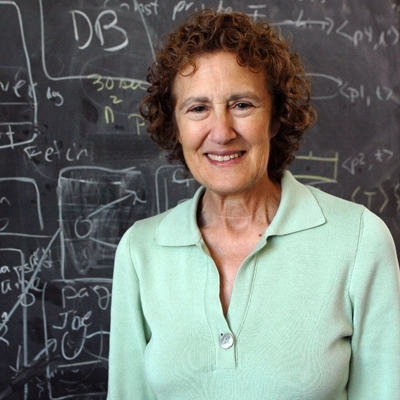
\includegraphics{barbara-liskov}}\\
        Barbara Liskov
      \end{center}
    \end{minipage}
  \end{center}
\end{slide}

\begin{slide}
  \pdfbookmark[1]{Interface Segregation}{interface-segregation}
  \pdfbookmark[2]{Before}{interface-segregation-before}
  \heading{Interface Segregation - Before}
  \begin{center}
    \begin{minted}{clojure}
(defrecord AccountHolder [name age balance])

(defn is-adult [account-holder] (>= (:age account-holder) 18))

(defn deposit [account-holder amount]
  (update account-holder :balance + amount))

(defn withdraw [account-holder amount]
  (update account-holder :balance - amount))
    \end{minted}
  \end{center}
\end{slide}

\begin{slide}
  \pdfbookmark[2]{After}{interface-segregation-after}
  \heading{Interface Segregation - After}
  \begin{center}
    \begin{minted}{clojure}
(defrecord Person [name age])

(defn is-adult [person]
  (>= (:age person) 18))

(defrecord Account [balance])

(defn deposit [account amount]
  (update account :balance + amount))

(defn withdraw [account amount]
  (update account :balance - amount))

(defrecord AccountHolder [person account])
    \end{minted}
  \end{center}
\end{slide}

\begin{slide}
  \pdfbookmark[1]{Dependency Inversion}{dependency-inversion}
  \pdfbookmark[2]{Before}{dependency-inversion-before}
  \heading{Dependency Inversion - Before}
  \begin{center}
    \begin{minted}{clojure}
(defn print-names [people print-writer]
  (doseq [person people]
         (.println print-writer (:name person))))
; ...
(print-names [{:name "Alice"} {:name "Bob"}] *out*)
    \end{minted}
  \end{center}
\end{slide}

\begin{slide}
  \pdfbookmark[2]{After}{interface-segregation-after}
  \heading{Dependency Inversion - After}
  \begin{center}
    \begin{minted}{clojure}
(defn print-names [people writer]
  (doseq [person people]
         (.write writer (:name person))
         (.write writer "\n")))
; ...
(print-names [{:name "Alice"} {:name "Bob"}] *out*)
; ...
(with-open [f (java.io.FileWriter. "names.txt")]
  (print-names [{:name "Alice"} {:name "Bob"}] f))
    \end{minted}
  \end{center}
\end{slide}

\begin{slide}
  \pdfbookmark[1]{Aspects of a Class}{class-aspects}
  \heading{Aspects of a Class}
  \begin{center}
    \textbf{The 5 aspects of the class are:}\footnote{\href{https://swarch.blog/the-five-principles-for-solid-software-design/}{Mike Lindner: The Five Principles For SOLID Software Design}}\\
    \resizebox*{.6\textwidth}{!}{
\includegraphics{aspects}}
  \end{center}
\end{slide}

\begin{slide}
  \pdfbookmark[1]{Principles of a Class}{class-aspects}
  \heading{The 5 Principles}
  \begin{center}
    \textbf{The 5 corresponding principles are:}\footnote{\href{https://swarch.blog/the-five-principles-for-solid-software-design/}{Mike Lindner: The Five Principles For SOLID Software Design}}\\
    \resizebox*{.6\textwidth}{!}{
\includegraphics{principles}}
  \end{center}
\end{slide}

\begin{slide}
  \pdfbookmark[1]{Thanks}{thanks}
  \heading{\ }
  \begin{center}
    \begin{Huge}
      Thanks
    \end{Huge}
  \end{center}
\end{slide}

\end{document}
